%%
%% This is file `sample-sigconf.tex',
%% generated with the docstrip utility.
%%
%% The original source files were:
%%
%% samples.dtx  (with options: `all,proceedings,bibtex,sigconf')
%% 
%% IMPORTANT NOTICE:
%% 
%% For the copyright see the source file.
%% 
%% Any modified versions of this file must be renamed
%% with new filenames distinct from sample-sigconf.tex.
%% 
%% For distribution of the original source see the terms
%% for copying and modification in the file samples.dtx.
%% 
%% This generated file may be distributed as long as the
%% original source files, as listed above, are part of the
%% same distribution. (The sources need not necessarily be
%% in the same archive or directory.)
%%
%%
%% Commands for TeXCount
%TC:macro \cite [option:text,text]
%TC:macro \citep [option:text,text]
%TC:macro \citet [option:text,text]
%TC:envir table 0 1
%TC:envir table* 0 1
%TC:envir tabular [ignore] word
%TC:envir displaymath 0 word
%TC:envir math 0 word
%TC:envir comment 0 0
%%
%%
%% The first command in your LaTeX source must be the \documentclass
%% command.
%%
%% For submission and review of your manuscript please change the
%% command to \documentclass[manuscript, screen, review]{acmart}.
%%
%% When submitting camera ready or to TAPS, please change the command
%% to \documentclass[sigconf]{acmart} or whichever template is required
%% for your publication.
%%
%%
\documentclass[sigconf]{acmart}

\usepackage{subcaption}
\usepackage{algorithm}
\usepackage{algpseudocode}

%%
%% \BibTeX command to typeset BibTeX logo in the docs
\AtBeginDocument{%
  \providecommand\BibTeX{{%
    Bib\TeX}}}



%%
%% Submission ID.
%% Use this when submitting an article to a sponsored event. You'll
%% receive a unique submission ID from the organizers
%% of the event, and this ID should be used as the parameter to this command.
%%\acmSubmissionID{123-A56-BU3}

%%
%% For managing citations, it is recommended to use bibliography
%% files in BibTeX format.
%%
%% You can then either use BibTeX with the ACM-Reference-Format style,
%% or BibLaTeX with the acmnumeric or acmauthoryear sytles, that include
%% support for advanced citation of software artefact from the
%% biblatex-software package, also separately available on CTAN.
%%
%% Look at the sample-*-biblatex.tex files for templates showcasing
%% the biblatex styles.
%%

%%
%% The majority of ACM publications use numbered citations and
%% references.  The command \citestyle{authoryear} switches to the
%% "author year" style.
%%
%% If you are preparing content for an event
%% sponsored by ACM SIGGRAPH, you must use the "author year" style of
%% citations and references.
%% Uncommenting
%% the next command will enable that style.
%%\citestyle{acmauthoryear}


%%
%% end of the preamble, start of the body of the document source.
\begin{document}

%%
%% The "title" command has an optional parameter,
%% allowing the author to define a "short title" to be used in page headers.
\title{A Complete High Performance Simulation and Rendering Pipeline for Fluid}

%%
%% The "author" command and its associated commands are used to define
%% the authors and their affiliations.
%% Of note is the shared affiliation of the first two authors, and the
%% "authornote" and "authornotemark" commands
%% used to denote shared contribution to the research.
\author{Quanquan Peng}
\authornote{Both authors contributed equally to this research.}
\email{bartholomew@sjtu.edu.cn}
\orcid{0000-0003-0666-998}
\affiliation{%
  \institution{Shanghai Jiao Tong University}
  \city{Shanghai}
  \country{China}
}
\author{Yiyu Liu}
\orcid{0009-0000-6852-1978}
\authornotemark[1]
\email{liu_yiyu@sjtu.edu.cn}
\affiliation{%
  \institution{Shanghai Jiao Tong University}
  \city{Shanghai}
  \country{China}
}

%%
%% By default, the full list of authors will be used in the page
%% headers. Often, this list is too long, and will overlap
%% other information printed in the page headers. This command allows
%% the author to define a more concise list
%% of authors' names for this purpose.
\renewcommand{\shortauthors}{Trovato et al.}

%%
%% The abstract is a short summary of the work to be presented in the
%% article.
\begin{abstract}
  Simulating and rendering fluid in real time has a lot of challenges. The simulation and rendering must be very efficient while keeping the quality. On top of that, we need to exploit the computing power as much as possible by parallelizing the calculation.

  We design and implement a complete simulation and rendering pipeline for fluid. We leverage the computational power by means of parallelization with Taichi framework~\cite{hu2019taichi, hu2019difftaichi, hu2021quantaichi}. With PBF, screen-based method and Layered Neighborhood Method optimization, we can achieve about 30 FPS with CUDA on a commercial laptop (RTX 3060 Laptop).
\end{abstract}

%%
%% The code below is generated by the tool at http://dl.acm.org/ccs.cfm.
%% Please copy and paste the code instead of the example below.
%%
\begin{CCSXML}
<ccs2012>
<concept>
<concept_id>10010147.10010371.10010352.10010379</concept_id>
<concept_desc>Computing methodologies~Physical simulation</concept_desc>
<concept_significance>500</concept_significance>
</concept>
<concept>
<concept_id>10010147.10010371.10010372</concept_id>
<concept_desc>Computing methodologies~Rendering</concept_desc>
<concept_significance>500</concept_significance>
</concept>
</ccs2012>
\end{CCSXML}

\ccsdesc[500]{Computing methodologies~Physical simulation}
\ccsdesc[500]{Computing methodologies~Rendering}
%%
%% Keywords. The author(s) should pick words that accurately describe
%% the work being presented. Separate the keywords with commas.
\keywords{Fluid Simulation, Fluid Rendering, Screen-space Rendering}
%% A "teaser" image appears between the author and affiliation
%% information and the body of the document, and typically spans the
%% page.


%%
%% This command processes the author and affiliation and title
%% information and builds the first part of the formatted document.
\maketitle

\section{Introduction}
Simulating fluid is by no means easy --- fluid are continuous while computers are only good at discrete things.
Generally, we use Naiver-Stokes Equation~\cite{navier1838navier} to describe fluid.
However, the way of representing fluid is a great problem that remains to be solved.
There are basically two kinds of approaches to represent fluid --- \textit{grid-based}~\cite{harlow1965numerical, foster2001practical} and \textit{particle-based}~\cite{monaghan1992smoothed, muller2003particle, antoci2007numerical, solenthaler2009predictive, macklin2013position}.
The former one uses girds with attributes of density and velocity that represent all the particles in the square or cube, while the latter one uses particles as elements in free-surface flow simulations.
\textit{Grid-based} simulation is better in terms of simulation speed but results in bad fidelity.
We will go into details in related works section.
In our work, we adopts \textit{particle-based} simulation to better represent the physical property of fluid.

As for the rendering methodology, there are roughly three types of rendering methods -- \textit{mesh-based}~\cite{solenthaler2007unified, adams2007adaptively}, \textit{ray-casting}~\cite{fraedrich2010efficient, zirr2015memory} and \textit{screen-based}~\cite{cords2009interactive, bagar2010layered, oliveira2022narrow}, each of which has its pros and cons. In brief, \textit{mesh-based} methods require high-resolution grid and turn out to be computationally expensive; \textit{ray-casting} methods also require enormous computational power; \textit{screen-based} methods is easier for computation but may emit some details. We will discuss about the details later. We adopts \textit{screen-based} method to ensure better rendering speed.

In our work, we design and implement a complete simulation and rendering pipeline for fluid. We leverage the computational power by means of parallelization with Taichi framework~\cite{hu2019taichi, hu2019difftaichi, hu2021quantaichi}. With PBF, screen-based method and Layered Neighborhood Method optimization, we can achieve about 30 FPS with CUDA on a commercial laptop (RTX 3060 Laptop). To our knowledge, this maybe one of the few (or even the first) open-sourced and light-weighted full-stack fluid simulation and rendering pipeline which supports GPU. Our source code is publicly available at \url{https://github.com/LauYeeYu/fluid-rendering/}.

\section{Related Works}
\subsection{Fluid Simulation methods}
We can generally divide the methodology in fluid simulation into two types --- \textit{grid-based} and \textit{particle-based} methods.

\textbf{Grid-based Methods.} In grid-based methods, every grid has its own attributes to represent the average property of all fluid in that grid~\cite{harlow1965numerical, foster2001practical}. Fluid is simulated in the view of flow field. The scale of the grid number largely limits accuracy of simulation. Generally, the grid number is less than the particle number in particle-based methods, so grid-based methods are faster in simulation speed but worse in fidelity.

\textbf{Particle-based methods.} Fluid is regarded as a collection of particles in particle-based methods, where simulation is achieved by calculating the force on each particle and simulating its movement. Smoothed Particle Hydrodynamics (SPH)~\cite{monaghan1992smoothed} is a well-established technique, celebrated for its mass conservation and adaptability in dynamic environments such as video games. Despite its advantages, SPH is susceptible to density fluctuations and the computational cost of enforcing incompressibility due to its unstructured nature. Advancements like Predictive-corrective Incompressible SPH (PCISPH)~\cite{solenthaler2009predictive} have enhanced real-time application feasibility by using iterative methods for gradual pressure convergence, allowing for larger time steps. Building on this, our work utilizes the Position Based Fluids (PBF)~\cite{macklin2013position} method, which integrates a position-based dynamics framework to address these challenges. PBF uses an iterative density solver to enforce constant density through positional constraints, combining the benefits of SPH incompressibility with the stability and efficiency of position-based methods, thereby enhancing the realism and performance of fluid simulations in real-time applications.

\subsection{Fluid Rendering Methods}
In the realm of screen-space fluid rendering, a variety of methods have been developed to efficiently render particle-based fluids in real-time applications. We can generally divide these methods into three types --- \textit{mesh-based}, \textit{ray-casting} and \textit{screen-based}.

\textbf{Mesh-based Methods.} These methods share the same core idea --- retrieve the surface mesh from the position of particles in the world-space coordinates. These methods use algorithms like Marching Cubes to get the mesh. These methods
can use isotropic kernels~\cite{solenthaler2007unified} or adaptive size kernels~\cite{adams2007adaptively}. However, retrieving the surface mesh and rendering based on the complicated mesh consumes excessive computing power and therefore not feasible for real-time rendering.

\textbf{Ray-casting Methods.} In ray-casting methods, the liquid surface is rendered by employing a GPU-based volume ray-casting of a scalar field defined from the fluid particles. \citet{fraedrich2010efficient} proposed an SPH particle rendering using an adaptive discretization of the view volume performing ray-casting in a perspective grid. With compression on the perspective grid by grouping the voxels, the memory consumption can be reduced~\cite{zirr2015memory}. However, although ray-casting methods allow interactive rendering, these techniques are unable to be applied on
real-time applications.

\textbf{Screen-space Methods.} These methods only cares about the frontmost surface and the distance of light in fluid, which affect the result of render most. In these methods, a scene is calculated into a depth buffer and a thickness buffer with perspective projection. After smoothened, these two buffers are converted into normal buffer and light attenuation value respectively. Traditional screen-space methods~\cite{cords2009interactive, bagar2010layered} rely on smoothing a depth buffer generated from particle data to create the visual representation of a fluid surface. These techniques, while effective in certain contexts, often require extensive computation, especially when using large convolution kernels or multiple filter passes, which can degrade performance significantly. A novel approach presented by Oliveira and Paiva~\cite{oliveira2022narrow} introduces a layered neighborhood method that significantly enhances performance by selectively processing only particles within a narrow band around the fluid's surface. This method not only reduces the computational load but also addresses speed deficiencies inherent in previous techniques that did not employ such an optimization. By focusing on boundary particles and effectively managing particle layers, the layered neighborhood method enables faster rendering times and reduces memory consumption, making it a robust solution for real-time fluid visualization in screen-space rendering frameworks.

\section{Simulation and Rendering Pipeline Design}

\subsection{Fluid Simulation}
\label{fluid-simulation}
Here we show how we do fluid simulation based on PBF method:

\textbf{Initialization:} Define and initialize particles that represent the fluid.

\textbf{Predict Position:}
\begin{itemize}
    \item Apply external forces such as gravity to update particle velocities.
    \item Predict future positions based on current velocities and time step.
\end{itemize}

\textbf{Constraint Enforcement:}
 Enforce density constraints to maintain fluid incompressibility through iterative position adjustments.

\textbf{Velocity Update:}
Update velocities based on the corrections made to positions during constraint enforcement.

\subsection{Fluid Rendering}
Since the particle positions are calculated in previous steps, we directly use these values and render the fluid.

\subsubsection{The Layer of each Particle}
Different from solid, fluid will gather together if are very close to each other. In this case, although the number of particles are large, only the outer particles are important for the shape of the fluid. As long as we know the shape of surface, we are able to restore almost every detail of the fluid accurately.

Then the question is, how to tell the outer particles from the inner particles? Since it is hard to exactly pick the nearby particles effeciently, we can divide the space into voxels and consider the voxels instead. The voxels that are likely to carry outer particles are considered as layer-1~\cite{oliveira2022narrow}. Notice that a voxel is layer-1 only when
\begin{enumerate}
\item it is on the boundary of the space;
\item it has at least one neighbor voxel without particles.
\end{enumerate}

For layer-2 voxel, a voxel is regarded as layer-2 if and only if
\begin{enumerate}
\item it is has particles in it;
\item it is not a layer-1 voxel;
\item it has at least on neighbor layer-1 voxel.
\end{enumerate}

Voxels with higher layer can be calculated similarly.

\subsubsection{Depth buffer}
With the preprocessed layer information, we can identify all the particles that are in layer-1 voxels. With these selected particles, we are able to generate the depth buffer since the frontmost particles must be the outer particles. We can simply map the particles to the place on the screen with perspective projection, and set the depth if the distance from the particle to the camera is less than the current value.

\subsubsection{Filtered Depth Buffer}
Now we've already got the depth information, but it is not enough. Since particles are discrete, the simple representation by spheres of the liquid surface will lead to an unrealistic blobby appearance. We need to smoothen and flatten the surface.

The filter method will be discussed in details in the implementation section.

\subsubsection{Normal Buffer}
With the smoothened normal buffer, we can generate the normal buffer easily. Just consider the change in value from up-down and left-right direction, we can calculate the normal of each screen pixel. The normal buffer is used for calculating the reflection of the frontmost surface.

\subsubsection{Thickness Buffer}
After computing the depth buffer, the inner particles are skipped by the remaining stages of the screen-space rendering pipeline. Therefore, we need to recover the fluid volume. To be specific, we need to estimate the thickness $T_{\mathcal{G}}$ using the voxels of $\mathcal{G}_h$.

Traditionally, we calculate the thickness by computing the contribution of each particle on each pixel. For each pixel $\overline{\mathbf{p}}$, the thickness from a particle set $\mathcal P$ is given by:
\begin{equation}
    T_{\mathcal P}\left(\overline{\mathbf{p}}\right) = \sum_{j=1}^{|\mathcal P|}G_{\sigma}\left(\left \lVert \overline{\mathbf{p}} - {\overline{\mathbf{x}}}_j \right \rVert_2 \right),
\end{equation}
where $\mathbf{x}_j$ is the position of the particle $j$ and ${\overline{\mathbf{x}}}_j$ is its projection on the screen-space,
and $G_{\sigma}$ is the Gaussian kernel with a radius of influence $\sigma$ as user-defined parameter, such that $G_\sigma (x) = \exp \left(-x^2 / 2 \sigma^2\right)$.

In our case, we use voxels to calculate the thickness. Hence, the thickness is given similarly:
\begin{equation}
    T_{\mathcal G}\left(\overline{\mathbf{p}}\right) = \sum_{j=1}^{|\mathcal F_h|}n_j G_{\sigma}\left(\left \lVert \overline{\mathbf{p}} - {\overline{\mathbf{c}}}_j \right \rVert_2 \right),
\end{equation}
where $\mathbf c_j$ is the centroid of the voxel and $n_j$ is the number of particles in voxel $j$.

\subsubsection{Filtered Thickness Buffer}
Similar to the process on depth buffer, the thickness buffer also suffers from an unrealistic blobby appearance. We need to smoothen the thickness buffer.

\subsubsection{Light Attenuation}
Before calculating the lighting model, we render the fluid volume using some light attenuation model. The loss of light intensity when it propagates
in a liquid is directly proportional to the light path length. Therefore, the resulting color is given by $\overline{\mathbf{rgb}} = \mathbf{rgb}\cdot \exp (-\kappa l)$, where $\kappa$ is the attenuation coefficient.

Calculating the exact length of light is impossible under screen-based rendering. A common approach is to use the thickness as an approximation of the length of light in fluid.

\section{Implementation}

Our code is written in Python and Taichi~\cite{hu2019taichi, hu2019difftaichi, hu2021quantaichi}. Taichi is a parallel programming language for high-performance numerical computation, which uses multiple parallelization framework, e.g., OpenGL, CUDA, etc., as its backend.

\subsection{PBF}
Based on the pipeline described in Sec.~\ref{fluid-simulation}, we show the code in Alg.~\ref{alg:pbf}, where:
the density constraint $C_i$ on the $i$-th particle is defined using an equation of state: 
 \begin{equation}
     C_{i}(\mathbf{p}_{1},...,\mathbf{p}_{n})=\frac{\rho_{i}}{\rho_{0}}-1, \\
     \lambda_{i}=-\frac{C_{i}(\mathbf{p}_{1},...,\mathbf{p}_{n})}{\sum_{k}\left|\nabla_{{\mathbf{p}_{k}}}C_{i}\right|^{2}}
 \end{equation}
 
Note that we split the 3D space into grids in order to accelerate the process of finding particles' neighbors and used SDF (signed distance field) for boundary detection.
\begin{algorithm}
\caption{PBF Simulation Loop}
\begin{algorithmic}[1]
\State \textbf{for} all particles $i$ \textbf{do}
\State \quad Apply forces $\mathbf{v}_i \leftarrow \mathbf{v}_i + \Delta t \mathbf{f}_{\text{ext}}(\mathbf{x}_i)$ \Comment{$\mathbf{f}_{\text{ext}} \text{ is the external force}$}
\State \quad Predict position $\mathbf{x}^*_i \leftarrow \mathbf{x}_i + \Delta t \mathbf{v}_i$
\State \textbf{end for}
\State \textbf{for} all particles $i$ \textbf{do}
\State \quad Find neighboring particles $N_i(\mathbf{x}^*_i)$
\State \textbf{end for}
\State \textbf{while} iter $<$ solverIterations \textbf{do} \Comment{solverIterations is a hyper-param}
\State \quad \textbf{for} all particles $i$ \textbf{do}
\State \quad \quad Calculate $\lambda_i$
\State \quad \textbf{end for}
\State \quad \textbf{for} all particles $i$ \textbf{do}
\State \quad \quad Calculate $\Delta \mathbf{p}_i$
\State \quad \quad Perform collision detection and response
\State \quad \textbf{end for}
\State \quad \textbf{for} all particles $i$ \textbf{do}
\State \quad \quad Update position $\mathbf{x}^*_i \leftarrow \mathbf{x}^*_i + \Delta \mathbf{p}_i$
\State \quad \textbf{end for}
\State \textbf{end while}
\State \textbf{for} all particles $i$ \textbf{do}
\State \quad Update velocity $\mathbf{v}_i \leftarrow \frac{1}{\Delta t} (\mathbf{x}^*_i - \mathbf{x}_i)$
\State \quad Apply vorticity confinement and XSPH viscosity
\State \quad Update position $\mathbf{x}_i \leftarrow \mathbf{x}^*_i$
\State \textbf{end for}
\end{algorithmic}
\label{alg:pbf}
\end{algorithm}


\subsection{LNM}
%TODO: LNM
Layered Neighborhood Method (LNM)~\cite{oliveira2022narrow} is the method used to accelerate the generation of the depth buffer. The key idea is that not all particles contribute to the depth buffer, only the out-layer does. The layers are determined by the k-ring neighborhood $\mathcal N_k(V)$ of a voxel $V$, as follows:
\begin{itemize}
    \item 0-ring is the voxel V itself;
    \item  The $k$-ring (with $k \in \mathbb N^*$) of $V$ is the set of adjacent voxels in its $(k-1)$-ring.
\end{itemize}
Define the distance of two voxels as:
\begin{equation}
\operatorname{dist}(V_i,V_j)=\min\{k\in\mathbb{N}\mid V_i\in\mathcal{N}_k(V_j)\}
\end{equation}
Note the set of empty voxels as $\mathcal{E}_h$ and level-set $\mathcal L_k:=\{V:\ell_i(V)=k\}$, where $\ell(V_i)=\begin{cases}\min_{E\in\mathcal{E}_h}\left\{\operatorname{dist}(V_i,E)\right\},&\text{if }V_i\text{ is not border}\\1,&\text{otherwise}\end{cases}.$ The pseudocode is described in Alg.~\ref{alg:lnm}, here we only consider $\mathcal L_1$ particles.

\begin{algorithm}
\caption{Layered Neighborhood Method (LNM)}
\begin{algorithmic}[1]
\Require $P, G_h, \text{dim}$
\Ensure narrow-band $B$
\State $B \leftarrow \emptyset$
\State $n_{\text{min}} \leftarrow 2^{\text{dim}}$
\ForAll{voxel $V_i \in G_h$}
    \State $n_i \leftarrow$ number of particles of $P$ inside $V_i$
    \State $\ell_i \leftarrow 0$
\EndFor
\ForAll{full voxel $V_i \in G_h$} \Comment{first layer}
    \If{$|N_i(V_i)| \neq 3^{\text{dim}}$} \Comment{$V_i$ is border}
        \State $\ell_i \leftarrow 1$
    \Else
        \ForAll{voxel $V_j \in \mathcal N_i(V_i)$}
            \If{$n_j = 0$} \Comment{$V_j$ is empty}
                \State $\ell_i \leftarrow 1$
                \State \textbf{break}
            \EndIf
        \EndFor
    \EndIf
\EndFor
\ForAll{full voxel $V_i \in G_h$} \Comment{second layer}
    \If{$\ell_i = 1$}
        \ForAll{voxel $V_j \in \mathcal N_i(V_i)$}
            \If{$\ell_j = 1$ and $n_j \leq n_{\text{min}}$}
                \State $\ell_i \leftarrow 2$
                \State \textbf{break}
            \EndIf
        \EndFor
    \EndIf
\EndFor
\ForAll{full voxel $V_i \in G_h$}
    \If{$\ell_i \neq 0$}
        \State $P_i \leftarrow$ particles of $P$ inside $V_i$
        \State $B \leftarrow B \cup P_i$
    \EndIf
\EndFor
\State \textbf{return} $B$
\end{algorithmic}
\label{alg:lnm}
\end{algorithm}


\subsection{Smoothening Filters}
\begin{figure*}[htb]
  \centering
  \subcaptionbox{Original depth buffer.}{
    
\includegraphics[page=21, width=0.3\textwidth]{Direct3D_Effects.pdf}
  }
  \hspace{1em}
  \subcaptionbox{Filtered by Gaussian blur filter.}{
    
\includegraphics[page=22, width=0.3\textwidth]{Direct3D_Effects.pdf}
  }
  \hspace{1em}
  \subcaptionbox{Filtered by bilateral filter.}{
    
\includegraphics[page=28, width=0.3\textwidth]{Direct3D_Effects.pdf}
  }
  \caption{The effect of Gaussian blur filter and bilateral filter on depth buffer.}
  \Description{The effect of Gaussian blur filter and bilateral filter on depth buffer.}
  \label{filters}
\end{figure*}

We have already discussed about the necessarity of smoothening filters in the rendering pipeline. A naive approach is to use Gaussian blur filter. This filter smoothen the values by weighted average of the pixel and its surrounding ones. However, we still want to preserve the silhouette edges in depth image so that particles don't get blended into background surfaces~\cite{screennvidia}. The soultion is to use biteral filters:
\begin{equation}
  I^\text{filtered}(x) = \frac{1}{W_p} \sum_{x_i \in \Omega} I(x_i)f_r(\|I(x_i) - I(x)\|)g_s(\|x_i - x\|),
\end{equation}
and the normalization term, $W_{p}$, is defined as
\begin{equation}
  W_p = \sum_{x_i \in \Omega}{f_r(\|I(x_i) - I(x)\|)g_s(\|x_i - x\|)},
\end{equation}
where
\begin{itemize}
  \item ${I^{\text{filtered}}}$ is the filtered image;
  \item $I$ is the original input image to be filtered;
  \item $x$ are the coordinates of the current pixel to be filtered;
  \item $\Omega$ is the window centered in $x$, so $x_{i}\in \Omega$ is another pixel;
  \item $f_{r}$ is the range kernel for smoothing differences in intensities (this function can be a Gaussian function);
  \item $g_{s}$ is the spatial (or domain) kernel for smoothing differences in coordinates (this function can be a Gaussian function).
\end{itemize}

Figure~\ref{filters} shows the result of each filters. From the figure, we can clearly find that particles are blended into background surfaces with Gaussian blue filter, while the silhouette edges are preserved with bilateral filter.

\section{Result}
\begin{figure*}[htb]
  \centering
  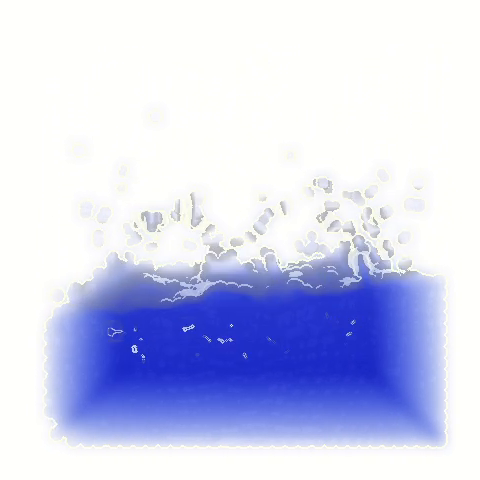
\includegraphics[width=0.4\textwidth]{result-1.png}
  \hspace{5em}
  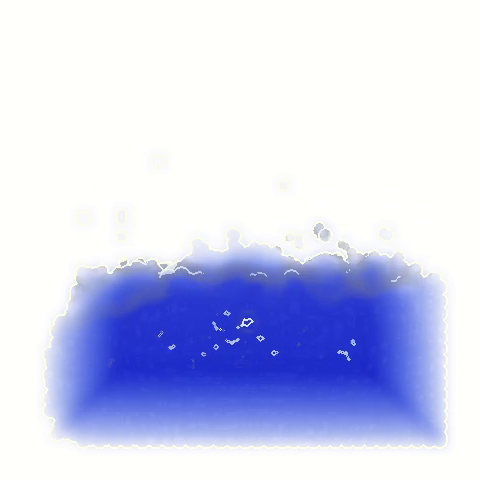
\includegraphics[width=0.4\textwidth]{result-2.png}
  \caption{Screenshots of the rendered fluid.}
  \Description{Results}
  \label{rendered-result}
\end{figure*}

\subsection{Experiment Setup}
We run simulation and rendering on a commercial laptop equipped with Intel Core i7-11800H and NVIDIA 3060 Laptop. The number of particles is set to 12,000.

\subsection{Performance}
With LNM method, we can achieve about 30 FPS with CUDA backend, and about 2.6 FPS with OpenGL backend. As a comparison, the frame per second with CUDA is only about 20 FPS, and 2.4 FPS with OpenGL.

Figure~\ref{rendered-result} shows the screenshots of the rendered fluid.

\subsection{Flaws}

\begin{figure}[htb]
  \centering
  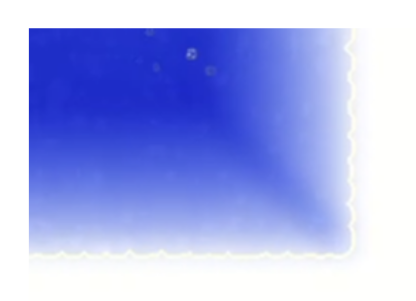
\includegraphics[width=0.4\textwidth]{flaw_1.png}
  \caption{Jagged edges. This is because the bilateral filter cannot smoothen the edges well.}
  \Description{Jagged edges}
  \label{jagged-edges}
\end{figure}

\begin{figure}[htb]
  \centering
  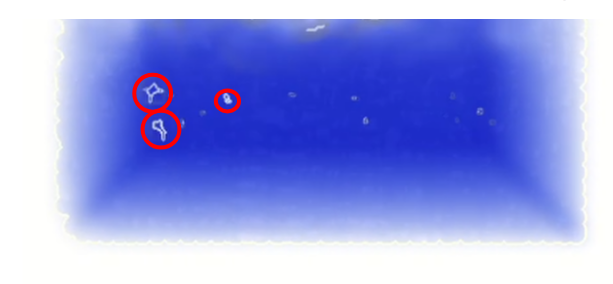
\includegraphics[width=0.4\textwidth]{flaw_2.png}
  \caption{Phantoms. This is because some critical particles are emitted with LNM.}
  \Description{Phantoms}
  \label{phantoms}
\end{figure}

Despite the result of render meets the frame per second of a real-time application, we found some flaws in the experiments.

Figure~\ref{jagged-edges} shows the jagged edges in rendering. This results from the bilateral filter. Although the bilateral filter is much better than the Gaussian blur in terms of keeping different surfaces separated, it cannot smoothen the edges well, so the edges will look like a round particle.

Figure~\ref{phantoms} show the phantoms in rendering. This boils down to the fact that some critical particles are emitted with the Layered Neighborhood Method.

\section{Conclusion}

In brief, we design and implement a complete simulation and rendering pipeline for fluid with both CPU and GPU supported. We use PBF and screen-space method with LNM optimization, which improves the performance dramatically while minimizing the influence on fidelity. With the power of GPU, we make real-time simulation and rendering possible, despite some minor flaws in the final result. Layered Neighborhood method improves the frame per second by 50\% with GPU and 8.3\% with CPU.

\section{Future Works}

\textbf{Avoiding jagged edges.} Although the result has some jagged edges, we need to find a solution of both keeping different surfaces separated while smoothening the edges.

\textbf{Improving LNM.} The current LNM largely prune the computation of rendering. However, we think we can further improve the algorithm in terms of its efficiency and accuracy. Figure~\ref{phantoms} indicates that the LNM has some inaccurate assertions. On the other hand, we now need to loop through grid and particles for multiple times, which is costly.

\textbf{Amending each step in simulation and rendering.} The current simulation and rendering procedure is not perfect and has room for improvement. We believe that with improving it will further increase the number of frames per second.


%%
%% The acknowledgments section is defined using the "acks" environment
%% (and NOT an unnumbered section). This ensures the proper
%% identification of the section in the article metadata, and the
%% consistent spelling of the heading.
\begin{acks}
We sincerely thank Prof. Yang for his invaluable guidance and to TA Shulin Hong for her dedicated assistance throughout this project.
\end{acks}

%%
%% The next two lines define the bibliography style to be used, and
%% the bibliography file.
\bibliographystyle{ACM-Reference-Format}
\bibliography{reference}


%%
%% If your work has an appendix, this is the place to put it.
\appendix


\end{document}
\endinput
%%
%% End of file `sample-sigconf.tex'.
